\documentclass[12pt,a4paper]{article}

\usepackage[utf8]{inputenc}
\usepackage[ngermanb]{babel}
% \usepackage{alphabeta} 
\usepackage{algpseudocode}
\usepackage{algorithm}

\usepackage[pdftex]{graphicx}
\usepackage[top=1in, bottom=1in, left=1in, right=1in]{geometry}

\linespread{1.06}
\setlength{\parskip}{6pt plus2pt minus2pt}

\widowpenalty 10000
\clubpenalty 10000
\setcounter{tocdepth}{3}

\newcommand{\eat}[1]{}
\newcommand{\HRule}{\rule{\linewidth}{0.5mm}}

\usepackage[official]{eurosym}
\usepackage{enumitem}
\setlist{nolistsep,noitemsep}
\usepackage[hidelinks]{hyperref}
\usepackage{cite}
\usepackage{svg}
\usepackage{amsfonts}
\usepackage{tikz}
\usetikzlibrary{shapes}

\setlength{\parindent}{0pt}
    
\floatname{algorithm}{Prozedur}

\begin{document}

%===========================================================
\begin{titlepage}
\begin{center}

% Top 

% Title
%\HRule \\[0.4cm]
%\vspace{0.4cm}
\vspace*{2cm}
{ \LARGE 
  \textbf{InformatiCup 2021 - Profit}\\[0.4cm]
  Theoretische Ausarbeitung\\
}
%\HRule \\[1.5cm]
\vspace*{2cm}

% Author
{ \large
  RustEvangelismStrikeforce\\
    \vspace*{1cm}
    
\includegraphics[width=0.3\textwidth]{logo.png}\\
  Tobias Schmitz \\ \href{tobias.schmitz@student.uni-siegen.de}{tobias.schmitz@student.uni-siegen.de} \\
  Maik Romancewicz \\ \href{maik.romancewicz@student.uni-siegen.de}{maik.romancewicz@student.uni-siegen.de} \\
}
\vfill



% Bottom
 
\end{center}
\end{titlepage}

%\begin{abstract}
%\lipsum[1-2]
\addtocontents{toc}{\protect\thispagestyle{empty}}
%\end{abstract}
\newpage

%===========================================================
\tableofcontents
%\addtocontents{toc}{\protect\thispagestyle{empty}}
\thispagestyle{empty}
\newpage

\thispagestyle{empty}
\newpage

\setcounter{page}{1}
%===========================================================
%===========================================================

\section{Einleitung}
Beim InformatiCup 2023 war die Aufgabe, im Rahmen einer rundenbasierten Simulation einen Produktionsprozess zu optimieren. Als Eingabe für das zu entwickelnde Programm erhält man ein 2-dimensionales Feld mit bereits platzierten Deposits und Obstacles, eine Liste von Produkten deren Produktion gewisse Ressourcen (aus den Deposits) benötigt und deren Produktion eine gewisse Punktzahl erzielt als auch ein Rundenlimit in dem die Simulation abläuft. Auf dem besagten Feld gilt es unterschiedliche Bauteile zu platzieren welche Ressourcen abbauen, diese transportieren und schließlich Produkte herstellen um Punkte zu erzielen. Ziel war es ein Programm zu entwickeln welches innerhalb einer vorgegebenen Zeit eine Liste an zu platzierenden Bauteilen generiert welche möglichst viele Punkte erzielt, in möglichst wenigen Runden.


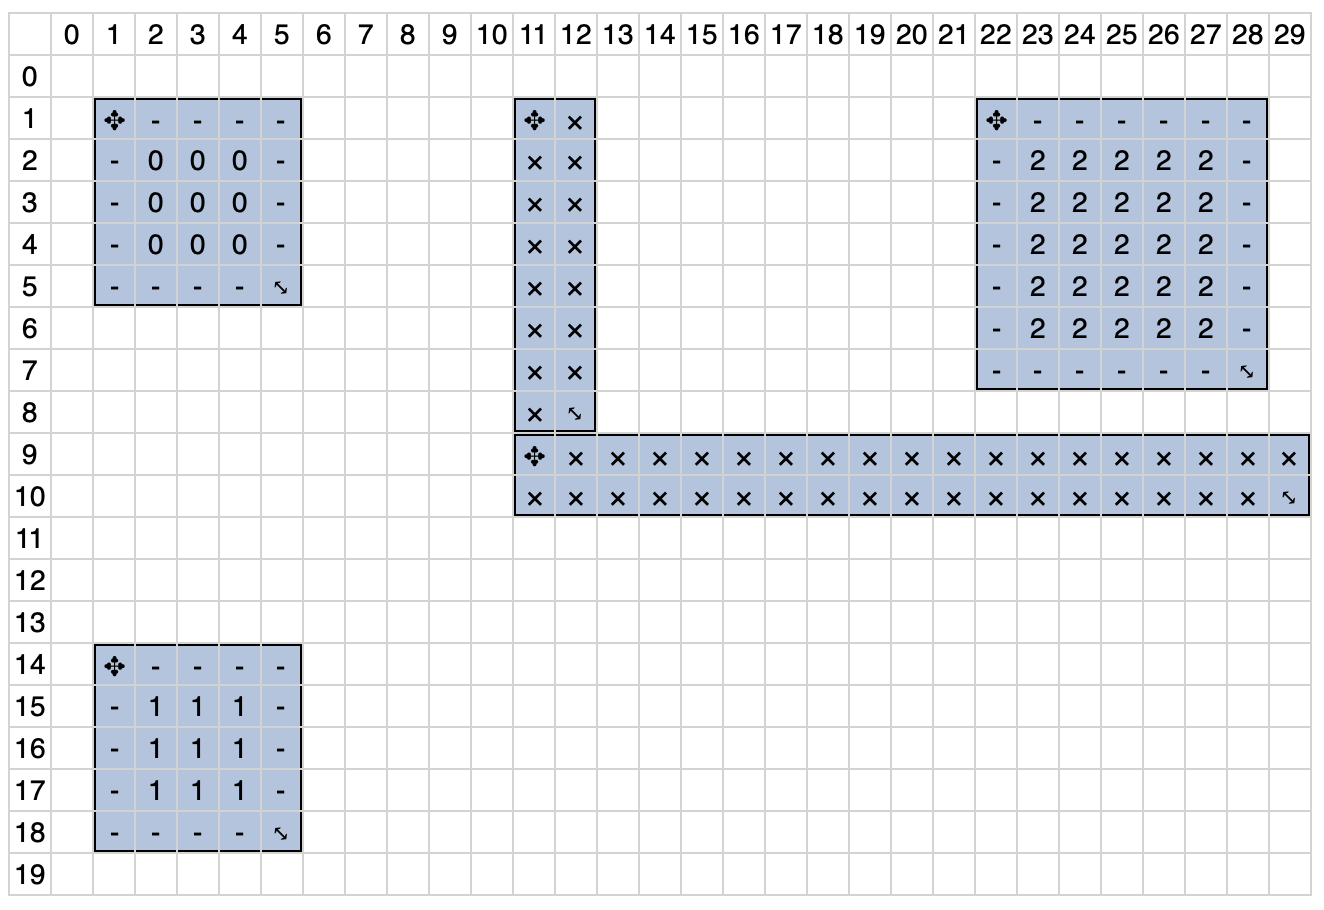
\includegraphics[width=\textwidth]{task1.png}

Eine ausführliche Beschreibung der Aufgabe ist auf der Website bzw. im Git Repository des Informaticups 2023 zu finden.

Wir werden in der folgenden Ausarbeitung anhand des obigen Beispiels erklären wie unsere Lösung funktioniert, welche Gedanken wir uns dazu gemacht haben und wie unser Programm letztendlich zu folgender Lösung kommt:

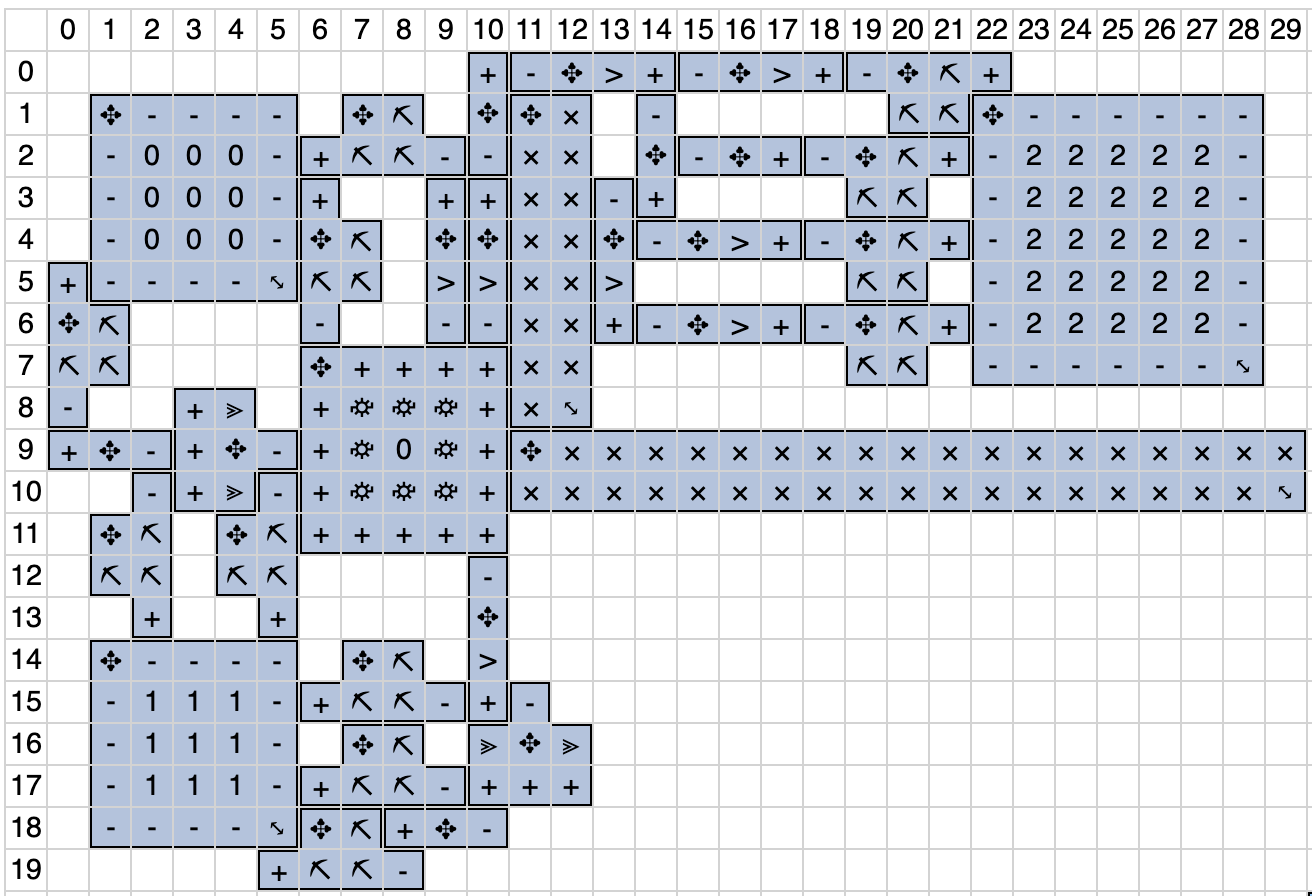
\includegraphics[width=\textwidth]{task1_solution.png}
% Lösungsbild einfügen

\section{Theoretischer Ansatz}
Im Laufe des Wettbewerbs hatten wir natürlich zahlreiche unterschiedliche Ideen wie man dieses Problem angehen kann und haben auch einige davon länger verfolgt. Letzten Endes sind wir zum Entschluss gekommen, dass wir die Aufgabenstellung in unterschiedliche Teilaufgaben unterteilen und versuchen diese einzeln anzugehen bevor wir die Erkenntisse die wir aus den Teilaufgaben gewonnen haben zu einer Gesamtlösung zusammenführen. Konkret bedeutet das, dass wir die Aufgabe in folgende Punkte unterteilt haben:

\begin{enumerate}
    \item Produktauswahl treffen
    \item Factory Platzierung
    \item Minen Platzierung
    \item Minen und Fabriken verbinden
\end{enumerate}

Die Idee hinter dieser Aufteilung war es, dass wir unsere Lösungen soweit Laufzeit-technisch optimieren, dass wir uns nicht auf einzelne Heuristiken verlassen müssen, sondern wir möglichst viele unterschiedliche Konfigurationen der Lösungen von den Teilaufgaben ausprobieren können. Dazu bringen wir die Lösungen der einzelnen Teilaufgaben in eine Rangliste und testen diese dann nacheinander kombiniert mit den Lösungen der anderen Teilaufgaben. Dazu brauchten wir also eine Simulationsumgebung mit der wir gefundene Lösungen testen können, Lösungsverfahren für die Einzelprobleme und eine sinnvolle Methode diese Lösungen miteinander zu kombinieren.

\newpage

\section{Implementierungen}

\subsection{Simulationsumgebung}
Das erste was wir zu Beginn des Wettbewerbs implementiert haben, ist eine Simulationsumgebung, die anhand einer Liste an Objekten die Simulation durchführt und uns die Punktzahl und die dafür benötigten Runden zurückgibt. (Angelehnt also an die letztendliche Abgabe unserer Lösung)

Damit haben wir uns zum Einen von der \href{profit.phinau.de}{Simulation} die uns für den Wettbewerb zur Verfügung gestellt wurde unabhängig gemacht und haben eine Simulationsumgebung die um ein Vielfaches schneller ist als die Web-basierte Implementierung auf der \href{profit.phinau.de}{profit.phinau.de} Website. Ursprünglich ist die Simulationsumgebung entstanden um als Supervision für Machine-Learning basierte Methoden (z.B als Reinforcement Learning environment) zu dienen. Bei diesen wäre es natürlich sehr wichtig gewesen, dass wir ggf. tausende Inputs schnell auswerten können, um unser Model zu trainieren. Allerdings haben wir unseren Ansatz im Laufe des Wettbewerbs geändert, trotzdem war die Simulationsumgebung ein integraler Bestandteil unserer Methodik. Mithilfe unserer Umgebung können wir einen gegebenen Input im Bruchteil einer Millisekunde auswerten und haben ein Feedback darüber wie gut die platzierten Bauteile die Aufgabe lösen.

%Implementierung weiter erklären

\subsection{Regionen}
Beim Ausführen unserer Lösung wird als Erstes die Umgebung in unterschiedliche Regionen unterteilt für den Fall, dass das Feld in mehrere Bereiche unterteilt wurde, die man nicht miteinander verbinden kann. 

Um diese Regionen zu finden laufen wir mithilfe eines rekursiven Path-finding Algorithmus einmal über das Feld und überprüfen für jedes Feld ob sich bereits ein Deposit oder ein Obstacle darauf befindet, falls wir ein Objekt finden werden die Felder mit einem Objekt aus der Eingabe gematched. Wenn alle Felder besucht wurden brechen wir ab, falls noch nicht alle Felder besucht wurden suchen wir an den umliegenden Stellen rekursiv weiter.

%Pseudocode

\newpage

\subsection{Distance Maps}
Als nächstes generieren wir für jedes Deposit eine Distance Map.
Eine Distance Map ist eine Map die für jede Zelle die Manhattan Distanz zu einem bestimmten Gebäude enthält.

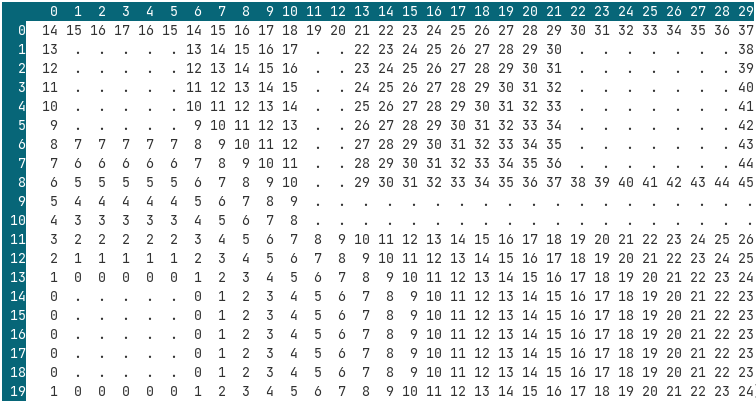
\includegraphics[width=\textwidth]{distance_map.png}


In dieser Distance Map zum Beispiel sehen wir die Distanzen von jeder Zelle zum Deposit unten links. Alle Zellen die als Punkt angezeigt werden sind mit Objekten belegt. Diese Distance Maps verwenden wir sowohl um die Factory zu platzieren, damit diese möglichst nah an bzw. möglichst gut zwischen den relevanten Deposits platziert wird und auch später um die kürzesten Wege von A nach B zu finden.

\subsection{Produkte filtern}
Als nächstes werden für jede Region anhand von einfachen Kriterien die Produkte gefiltert. Produkte die mehr Ressourcen oder andere Ressourcen benötigen als in einer Region vorhanden sind, können in dieser Region selbstverständlich nicht produziert werden.

\subsection{Deposits gewichten}
Nicht jede Ressource ist zur Produktion eines Produkts gleich wichtig. Wie viele Deposits  von einer Ressource zur Verfügung stehen, wie viele Ressourcen zur Produktion eines Produkts benötigt werden und auch wie viele Ressourcen pro Deposit zur Verfügung stehen muss mit in Betracht gezogen werden um eine sinnvolle Gewichtung der Deposits zu erstellen.

%Gewichtung Formel

Diese Gewichtung verwenden wir im nächsten Schritt um die Factory zu platzieren welche dann das gewünschte Produkt herstellt.

\subsection{Factory platzieren}
Zuerst werden alle Felder auf denen keine Factory platziert werden kann ausgefiltert und auch alle Factory Platzierungen die nicht alle nötigen Ressourcen rechtzeitig erhalten würden. Danach werden die möglichen Felder mithilfe der Deposit Gewichtung in eine Rangliste gebracht.
Folgende Scores werden berechnet, gewichtet und aufsummiert um eine Gesamtpunktzahl für die potenziellen Factory Positionen zu erhalten:

\begin{enumerate}
    \item Gesamtdistanz zu den Deposits
    \item Gewichtete Distanz zu den Deposits
    \item Differenz der Distanz zum nächsten Deposit und zum am weitesten entfernten Deposit
    \item Abschätzung wie viele Produkte an der Factory Position hergestellt werden können 
\end{enumerate}

An dieser Stelle könnte unsere Lösung noch weiter optimiert werden um über möglichst viele Aufgaben hinweg ein besonders gutes Ranking zu erstellen. Perfekt wäre ein Ranking welches immer an erster Stelle eine 'perfekte' Lösung hat. In diesem Fall wäre das also eine Factory Position mit der unsere restliche Lösung die maximale Punktzahl erreicht, die über alle Factory Positions hinweg erreicht werden kann. Vermutlich gibt es keine Gewichtung der vier oben genannten Kriterien, die für jede mögliche Aufgabe immer eine perfekte Factory an erster Stelle platziert. Allerdings kann man sich natürlich einer möglichst guten Gewichtung annähern in dem man über viele Aufgaben optimiert.

\subsection{Connection Tree}
Im nächsten Schritt passiert der Großteil unserer Lösung. Das Verbinden von Deposits und Factories mithilfe von Minen und den Verbindungsbausteinen. Wie bereits oben beschrieben basiert unsere Lösung in sehr großen Teilen möglichst effizient viele Möglichkeiten auszuprobieren und mit vielversprechenden Varianten weiter zu arbeiten. Vor Allem im Falle der Verbindungen ist dies sehr zum Tragen gekommen.

Unsere Lösung baut zunächst einen Baum aus Minen-Platzierungen und daran geknüpfte Verbindungenn mit einer Suchtiefe $n$ auf. Der beste Pfad in diesem Baum wird nach der Distanz des letzen Pfadsegments zu der Factory ausgewählt. Anschließend wird das erste Pfad Segment des besten Pfades platziert und von dort aus wird ein neuer Baum mit der Suchtiefe $n$ generiert.

Dazu iterieren wir über zahlreiche unterschiedliche Reihenfolgen unserer Deposits die wir mit unserer Factory verbinden wollen, platzieren wenn möglich eine Mine am Deposit und versuchen diese dann mithilfe unserer Distance Map Schritt für Schritt mit der Factory zu verbinden.

Bei der Implementierung wurde darauf geachtet, dass nur einmal zu Beginn ein ConnectionTree allocated wird, der Baum ist hierbei nicht Hierarchich strukturiert, sondern besteht im Grunde nur aus einem linearen Array, bestehend aus Nodes, welche die Indizes ihrer Children Nodes enthalten. Hierdurch ist die Implementierung sehr Cache-Freundlich.

%weiter ausführen 
%===========================================================

\newpage
\section{Verwendete Technologien}

\subsection{Rust}
Unsere Lösung haben wir vollständig in Rust implementiert. Da wir vor allem auf Performance gesetzt haben und alle Komponenten soweit wie möglich optimieren wollten und unsere Lösung  natürlich innerhalb eines Zeitlimits fertig werden musste, waren Sprachen mit Garbage-Collection ausgeschlossen. Rust hat es uns ermöglicht Code zu schreiben der das vorgegebene Problem effizient und schnell löst.

\subsection{GitHub}
Wir haben GitHub zum einen natürlich für die Zusammenarbeit während des Wettbewerbs verwendet, als auch um die Möglichkeiten von GitHub Actions zu nutzen.


\section{Softwarearchitektur}
Unsere Software Architektur legt Wert auf Wiederverwendbarkeit der einzelnen Komponenten. So sind die Komponenten, welche die eigentliche Logik zur Simulation und Lösung der Aufgaben, als Rust 'crates' definiert, und das CLI welches im Wettbewerb die Eingabe und Ausgabe behandelt, ruft diese bloß auf. Somit könnte ohne weitere Umstände eine GUI, oder ein Web-Server auf die gleichen Logikbausteine zurückgreifen ohne diese neu strukturieren oder kopieren zu müssen.

Die einzelen 'Crates' legen viel Wert auf Data-Driven Design statt durch undurchsichtige Objekt-Strukturen, den Fluss der Daten zu verschleiern. Obwohl für einzelne Datenstrukturen Methoden benutzt wurden, meist für simplere Zugriffe oder Berechnungen, sind die eigentlich tragenden Algorithmen meist in einfachen Funktionen umgesetzt und ein Blick auf deren Signatur lässt erkennen welche Daten benötigt und zurückgegeben werden.

\section{Software Testing}
Beim Testing greifen wir auf das in Rust standardmäßig enthaltene Testing-Framework zurück. Es wurden sowohl Unit-Tests für einzelne Komponenten, als auch Integrations-Tests wie z.B. für die ganze Simulation geschrieben. Viele dieser Tests enstanden aus Bug-Hunts und verhindern Regressionen beim Refactoring des existierenden Codes. Diese Tests werden zusätzlich auf GitHub via CI Actions automatisch bei jedem 'Push' ausgeführt.

\newpage

\section{Coding Conventions}
Die Coding Conventions lehnen sich hauptsächlich an die in großen Teilen der Rust-Community etablierten Standards an. So wurde zur Formattierung des Codes z.B. 'rustfmt' genutzt.
Um mögliche Bugs durch Verwechslung zu vermeiden wurde für häufig verwendete Indizes das New-Type Pattern angwendet. Die Indizes in den Bauteil Arrays der Simulation sind ein Tupel-Struct welches einen 16bit Integer enthält, Da beim Zugreifen auf dieses Array der genaue Datentyp erfordert wird, kann es nicht zu Verwechslungen mit zu anderen Datenstrukturen zugehörigen Indizes kommen.
Da von Anfang an Performance im Mittelpunkt stand, wurde bei allen Datentypen darauf geachtet so wenig wie möglich Speicher in Anspruch zu nehmen, um dem Compiler bei der automatischen Vektorisierung durch SIMD Instruktionen in die Hände zu spielen und die größtmögliche Menge an relevanten Daten im Cache bereitstehen zu haben. So ist der Koordinaten Datentyp nur 2 Byte groß, da dies bereits das maximal 100x100 große Spielfeld abdeckt. Ressourcen sind in einem 8-elementigen Array bestehend aus 16bit Integern gespeichert, so können simple arithmetische Operationen von zwei Resourcen-Arrays mit einer einzigen MMX Instruktion durchgeführt werden.

\section{Fazit}

Mithilfe unserer theoretischen Ansätze und unserer performanten Implementierung dieser sind wir unserer Ansicht nach zu einer sehr guten Lösung der Aufgabe gelangt. Uns sind natürlich noch immer Schwächen unserer jetzigen Lösung bewusst. Allerdings ist unsere Abgabe in der Lage für  verschiedenste Inputs eine gute Lösung bzw. teilweise auch eine optimale Lösung zu finden.
\end{document} 
